\section{Data Analysis}

\subsection{Overview of the Analytical Dataset}

The analytical workflow combines three connected evidence layers: product-day sales snapshots, customer review records, and clustering outputs derived from product-level performance features. Instead of relying only on narrative description, this section begins with a compact profile of the prepared analytical dataset and then presents each objective through the dashboard visuals that were actually used in the final report.

\begin{table}[H]
\centering
\renewcommand{\arraystretch}{1.3}
\begin{tabular}{|l|r|}
\hline
\textbf{Indicator} & \textbf{Value} \\ \hline
Analytical rows & 18,523 \\ \hline
Unique products & 693 \\ \hline
Unique categories & 21 \\ \hline
Analytical days & 29 \\ \hline
Average rating score & 4.78 \\ \hline
Review rows & 7,605 \\ \hline
\end{tabular}
\caption{High-level profile of the analytical dataset}
\label{tab:dataset-profile}
\end{table}

Table \ref{tab:dataset-profile} shows that the prepared dataset is large enough to support all ten objectives in the report. The sales layer contains \textbf{18,523} product-day observations across \textbf{693} products and \textbf{21} categories over \textbf{29} analytical days, while the review layer contributes \textbf{7,605} customer review records. The revenue, price, rating, and stock indicators also confirm that the Nike Lazada portfolio is a mid-to-high-priced catalog with generally positive ratings and very limited out-of-stock behavior during the observed period.

\begin{table}[H]
\centering
\small
\renewcommand{\arraystretch}{1.3}
\begin{tabularx}{\textwidth}{|>{\ttfamily}p{0.27\textwidth}|p{0.19\textwidth}|X|}
\hline
\textbf{Component} & \textbf{Grain / Structure} & \textbf{Role in Analysis} \\ \hline
fact\_product\_snapshot & Product-date level & Main sales, price, stock, and rating layer \\ \hline
fact\_review & Individual review level & Customer feedback and review-signal layer \\ \hline
dim\_product & Product reference table & Product identity and product attributes \\ \hline
dim\_category & Category reference table & Category-level grouping and comparison \\ \hline
dim\_date & Shared calendar table & Time-based aggregation for both facts \\ \hline
dim\_shop & Shop reference table & Store-level context \\ \hline
product\_segments & Product-level cluster output & Machine-learning segmentation layer \\ \hline
\end{tabularx}
\caption{Analytical data structure used in Section 3}
\label{tab:data-structure}
\end{table}

From a structural perspective, the analytical dataset follows a star-schema style design centered on two fact tables. The first fact table, \texttt{fact\_product\_snapshot}, supports the sales-oriented objectives because it stores daily observations of revenue, units sold, price, discount rate, stock status, rating score, and review count at the product-date level. The second fact table, \texttt{fact\_review}, supports customer-feedback analysis because it stores individual review records with rating, comment, and timestamp information. These two facts are connected to shared dimensions for product, category, date, and shop, while \texttt{product\_segments} extends the model with clustering outputs for the machine learning objectives.

\begin{table}[H]
\centering
\small
\renewcommand{\arraystretch}{1.3}
\begin{tabularx}{\textwidth}{|>{\ttfamily}p{0.28\textwidth}|X|}
\hline
\textbf{Variable} & \textbf{Observed Distribution Summary} \\ \hline
selling\_price & Mean = 2.04 million VND; min = 309,000 VND; max = 6.18 million VND \\ \hline
daily\_units\_sold & Mean = 0.19; max = 134; 16,967 zero-sale rows vs 1,556 positive-sale rows \\ \hline
daily\_revenue & Mean = 320,460 VND per row; max = 164.02 million VND \\ \hline
rating\_score & Mean = 4.78 across rated observations; ratings available in 15,119 rows \\ \hline
is\_in\_stock & 99.55\% of product-day rows are in stock \\ \hline
review\_date & Review rows distributed across 2024--2026, with the largest volume in 2025 \\ \hline
\end{tabularx}
\caption{Distribution summary of the main analytical variables}
\label{tab:variable-distribution}
\end{table}

The variable distributions reveal several important properties of the dataset. First, the selling-price distribution confirms that the portfolio is concentrated in the mid-to-high price range, which is consistent with the finance structure objectives later in the report. Second, the \texttt{daily\_units\_sold} variable is sparse: most product-day rows record zero units sold, while a much smaller number of rows contain positive values and a few extreme peaks. This means the sales pattern is uneven and supports the need for trend and concentration analysis. Third, the \texttt{rating\_score} and stock variables are both highly favorable overall, with a high mean rating and an in-stock ratio close to 100\%. Finally, the review data are not evenly distributed by year, because most of the collected customer-review records fall in 2025, which is important when interpreting the monthly review visuals in Theme 4.

\subsection{Theme 1: Sales Performance by Category and Time}

\subsubsection{Objective 1.1: Total Revenue by Category Name (Column Chart)}
\begin{figure}[H]
    \centering
    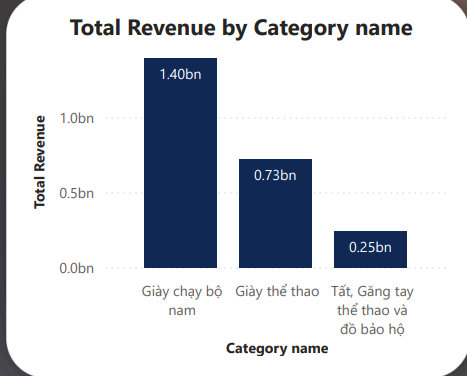
\includegraphics[width=0.72\textwidth]{images/1.1.png}
    \caption{Total revenue by category name}
\end{figure}

\begin{itemize}[leftmargin=*, label=\textbullet]
    \item \textbf{Mark:} Vertical bars.
    \item \textbf{Channel:} Bar height encodes total revenue as a quantitative measure, the X-axis position encodes category name as a categorical field, and text labels on bars reinforce exact values.
    \item \textbf{Rationale:} This chart was chosen because Objective 1.1 asks which categories contribute the most total revenue. A column chart answers that objective clearly by placing all categories on a common baseline, allowing direct comparison of revenue magnitude across groups.
    \item \textbf{Insight:} Revenue is clearly concentrated in a small number of categories. \textit{Giay chay bo nam} leads with about \textbf{1.40 billion VND}, followed by \textit{Giay the thao} at \textbf{0.73 billion VND}, while the third category contributes much less at about \textbf{0.25 billion VND}. This indicates that short-term sales performance is driven primarily by a narrow set of core categories rather than by the full catalog evenly.
\end{itemize}

\subsubsection{Objective 1.2: Category Revenue Stability and Volatility (Horizontal Bar Charts)}
\begin{figure}[H]
    \centering
    \begin{subfigure}[t]{0.48\textwidth}
        \centering
        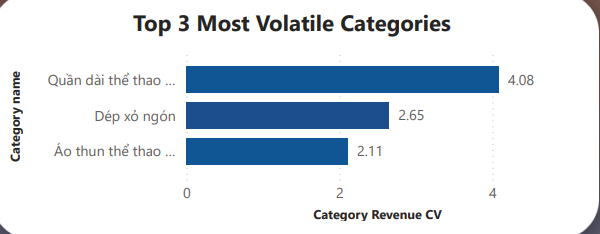
\includegraphics[width=\linewidth]{images/1.2 (1).png}
        \caption{Top 3 most volatile categories}
    \end{subfigure}
    \hfill
    \begin{subfigure}[t]{0.48\textwidth}
        \centering
        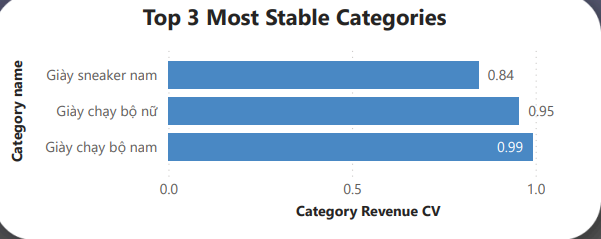
\includegraphics[width=\linewidth]{images/1.2 (2).png}
        \caption{Top 3 most stable categories}
    \end{subfigure}
    \caption{Category revenue CV comparison}
\end{figure}

\begin{itemize}[leftmargin=*, label=\textbullet]
    \item \textbf{Mark:} Horizontal bars.
    \item \textbf{Channel:} Bar length encodes \texttt{Category Revenue CV} quantitatively, the Y-axis position encodes category names categorically, and value labels show the relative degree of volatility or stability.
    \item \textbf{Rationale:} These charts were chosen because Objective 1.2 asks our group to identify and compare the most volatile and most stable categories. Horizontal bar charts answer that ranking task well by making coefficient-of-variation values easy to order, compare, and interpret side by side.
    \item \textbf{Insight:} The volatility pattern is uneven. The most volatile category reaches a CV of about \textbf{4.08}, far above the others, while the stable categories remain below \textbf{1.00}. In particular, \textit{Giay sneaker nam}, \textit{Giay chay bo nu}, and \textit{Giay chay bo nam} show relatively consistent performance, whereas categories such as long sports pants and flip-flops depend more heavily on short-lived revenue spikes.
\end{itemize}

\subsection{Theme 2: Finance Structure}

\subsubsection{Objective 2.1: Price Distribution by Price Band (Pie Chart)}
\begin{figure}[H]
    \centering
    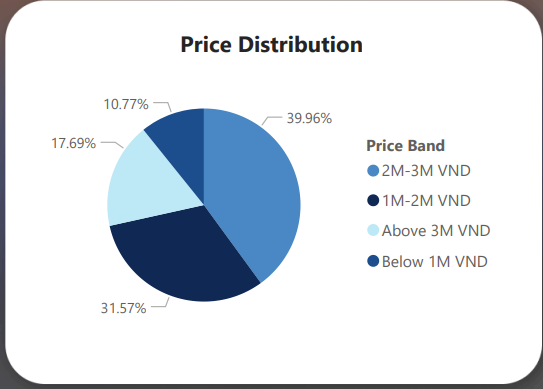
\includegraphics[width=0.72\textwidth]{images/2.1.png}
    \caption{Revenue distribution by price band}
\end{figure}

\begin{itemize}[leftmargin=*, label=\textbullet]
    \item \textbf{Mark:} Pie slices.
    \item \textbf{Channel:} Slice angle and area encode revenue share quantitatively, while color distinguishes the four categorical price bands.
    \item \textbf{Rationale:} This chart was chosen because Objective 2.1 focuses on part-to-whole comparison across a small number of price bands. A pie chart directly answers that objective by showing how total revenue is divided among the price groups and by making the dominant price band immediately visible.
    \item \textbf{Insight:} The portfolio's financial center lies in the middle price range. The \textbf{2M--3M VND} band contributes the largest share at about \textbf{39.96\%}, followed by the \textbf{1M--2M VND} band at \textbf{31.57\%}. The \textbf{Above 3M VND} and \textbf{Below 1M VND} groups contribute much smaller shares, so overall revenue is driven mainly by mid-priced products rather than extreme price segments.
\end{itemize}

\subsubsection{Objective 2.2: Top Trending Daily Revenue Pattern (Line Chart)}
\begin{figure}[H]
    \centering
    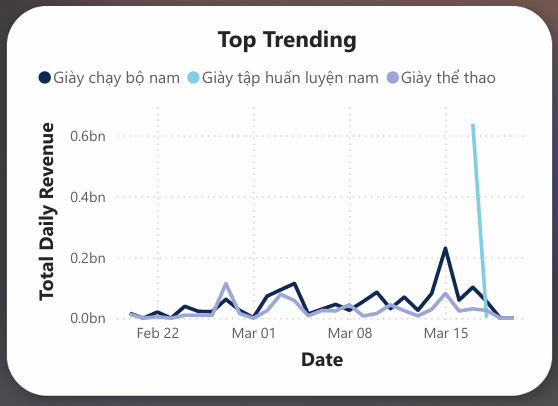
\includegraphics[width=0.78\textwidth]{images/2.2.png}
    \caption{Top trending categories by daily revenue}
\end{figure}

\begin{itemize}[leftmargin=*, label=\textbullet]
    \item \textbf{Mark:} Lines.
    \item \textbf{Channel:} Horizontal position encodes date, vertical position encodes total daily revenue, and color differentiates the leading categories shown in the chart.
    \item \textbf{Rationale:} This chart was chosen because Objective 2.2 asks whether revenue behavior is spread across time or concentrated on a small number of dates. A line chart answers that objective effectively by showing daily movement, sudden spikes, and differences in timing across the leading categories.
    \item \textbf{Insight:} Revenue movement is not evenly distributed across the period. Most dates remain at relatively low levels, but there are clear spikes in mid-March, especially for \textit{Giay tap huan luyen nam}, which rises sharply above the other categories. This suggests that page-level financial performance is shaped by a small number of high-impact dates rather than by smooth daily accumulation.
\end{itemize}

\subsection{Theme 3: Product Influence Analysis}

\subsubsection[Objective 3.1: Top Products by Average Unit Sold (Horizontal Bar Chart)]{Objective 3.1: Top Products by Average Unit Sold\texorpdfstring{\\}{ }(Horizontal Bar Chart)}
\begin{figure}[H]
    \centering
    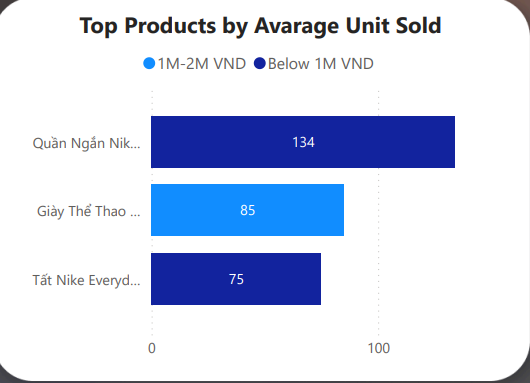
\includegraphics[width=0.72\textwidth]{images/3.1.png}
    \caption{Top products by average unit sold}
\end{figure}

\begin{itemize}[leftmargin=*, label=\textbullet]
    \item \textbf{Mark:} Horizontal bars.
    \item \textbf{Channel:} Bar length represents \texttt{Avg Daily Units Sold}, Y-axis position represents product identity, and color differentiates the associated price-band grouping shown in the legend.
    \item \textbf{Rationale:} This chart was chosen because Objective 3.1 asks which products lead unit performance. A horizontal bar chart answers that objective clearly by ranking products from strongest to weakest while also giving enough space for long product labels.
    \item \textbf{Insight:} Product influence is concentrated, but not fully monopolized by a single item. The leading product reaches about \textbf{134} average units sold, clearly ahead of the second product at \textbf{85} and the third at \textbf{75}. This shows that a small set of standout items plays an important role in unit performance, although there is still a noticeable spread across multiple top products.
\end{itemize}

\subsubsection{Objective 3.2: Top Product Unit Trend (Line Chart)}
\begin{figure}[H]
    \centering
    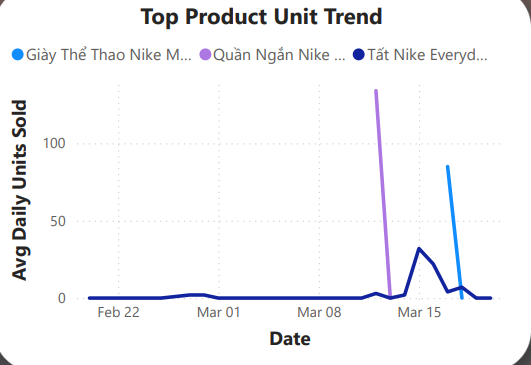
\includegraphics[width=0.72\textwidth]{images/3.2.png}
    \caption{Top product unit trend over time}
\end{figure}

\begin{itemize}[leftmargin=*, label=\textbullet]
    \item \textbf{Mark:} Lines.
    \item \textbf{Channel:} The X-axis represents date, the Y-axis represents \texttt{Avg Daily Units Sold}, and color separates the tracked top products.
    \item \textbf{Rationale:} This chart was chosen because Objective 3.2 asks whether top-product performance is stable over time or driven by a few spike dates. A line chart answers that objective better than a ranking chart because it preserves the time sequence and highlights sudden increases in units sold.
    \item \textbf{Insight:} The strongest products do not perform uniformly across the full period. Instead, the chart shows several sharp spikes in mid-March, including one product peaking above \textbf{130} units and another later peak near \textbf{85} units. This indicates moderate concentration risk: short-term product influence depends partly on a few strong surge dates rather than on perfectly stable demand.
\end{itemize}

\subsection{Theme 4: Customer Ratings and Review Signals}

\subsubsection[Objective 4.1: Monthly Rating and Review Trends (Dual-Axis Line Chart)]{Objective 4.1: Monthly Rating and Review Trends\texorpdfstring{\\}{ }(Dual-Axis Line Chart)}
\begin{figure}[H]
    \centering
    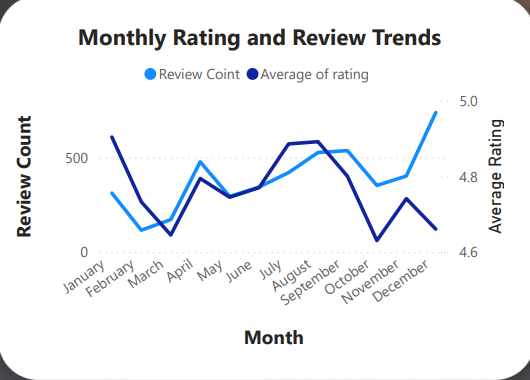
\includegraphics[width=0.72\textwidth]{images/4.1.png}
    \caption{Monthly rating and review trends}
\end{figure}

\begin{itemize}[leftmargin=*, label=\textbullet]
    \item \textbf{Mark:} Two lines on a dual-axis chart.
    \item \textbf{Channel:} The X-axis encodes month, the left Y-axis encodes review count, the right Y-axis encodes average rating, and color distinguishes the two measures.
    \item \textbf{Rationale:} This chart was chosen because Objective 4.1 asks our group to compare two monthly signals at the same time: review count and average rating. A dual-axis line chart answers that objective well by placing both measures on the same timeline while keeping their different numeric scales readable.
    \item \textbf{Insight:} Customer sentiment remains generally high, with the rating line staying in the upper 4.6 to 4.9 range, while review volume varies more noticeably by month. Review activity rises strongly in April and again toward December, whereas average rating dips more clearly around March and November. This means customer attention fluctuates more than customer satisfaction does.
\end{itemize}

\subsubsection[Objective 4.2: Monthly Comment Trends for Top Products (Line Chart)]{Objective 4.2: Monthly Comment Trends for Top Products\texorpdfstring{\\}{ }(Line Chart)}
\begin{figure}[H]
    \centering
    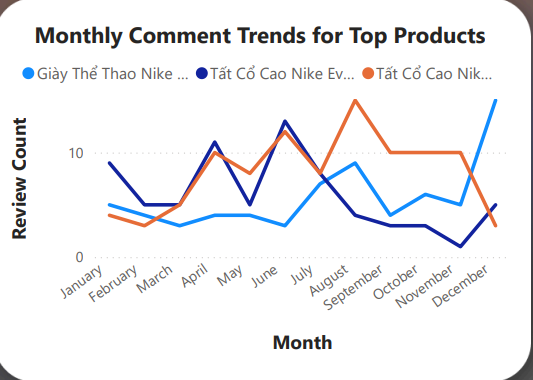
\includegraphics[width=0.72\textwidth]{images/4.2.png}
    \caption{Monthly comment trends for top products}
\end{figure}

\begin{itemize}[leftmargin=*, label=\textbullet]
    \item \textbf{Mark:} Lines.
    \item \textbf{Channel:} Horizontal position represents month, vertical position represents review count, and color differentiates the most-discussed products.
    \item \textbf{Rationale:} This chart was chosen because Objective 4.2 asks which products receive the most comments across months and whether that attention stays concentrated. A multi-line chart answers that objective clearly by showing changes in monthly leadership, persistence, and spikes for each tracked product.
    \item \textbf{Insight:} Customer discussion is not dominated by one product throughout the year. Different products lead in different months: one line peaks strongly in August, another becomes more prominent around June, and another jumps highest in December. This suggests that review attention rotates across products rather than remaining permanently concentrated in a single item.
\end{itemize}

\subsection{Theme 5: Machine Learning Insights (Clustering)}

\subsubsection{Objective 5.1: Clustering Quality and Segment Identification (Bar Chart and Scatter Plot)}
\begin{figure}[H]
    \centering
    \begin{subfigure}[t]{0.48\textwidth}
        \centering
        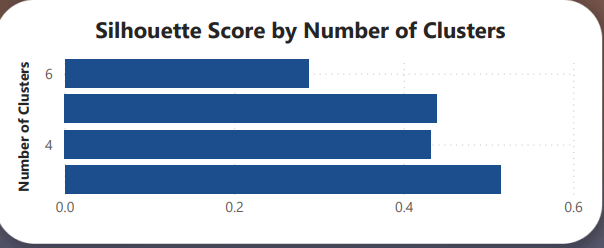
\includegraphics[width=\linewidth]{images/5.1.png}
        \caption{Silhouette score by number of clusters}
    \end{subfigure}
    \hfill
    \begin{subfigure}[t]{0.48\textwidth}
        \centering
        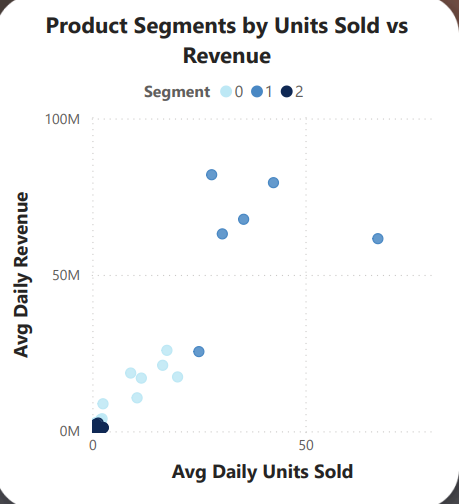
\includegraphics[width=\linewidth]{images/5.2 (1).png}
        \caption{Product segments by units sold vs revenue}
    \end{subfigure}
    \caption{Clustering quality and segment identification}
\end{figure}

\begin{itemize}[leftmargin=*, label=\textbullet]
    \item \textbf{Mark:} Horizontal bars in the silhouette chart and points in the scatter plot.
    \item \textbf{Channel:} In the first visual, bar length encodes silhouette score and Y-axis position encodes the candidate number of clusters. In the second visual, X-axis position encodes \texttt{Avg Daily Units Sold}, Y-axis position encodes \texttt{Avg Daily Revenue}, and color encodes cluster membership.
    \item \textbf{Rationale:} These charts were chosen because Objective 5.1 has two linked tasks: selecting a reasonable clustering solution and checking whether the resulting segments are visibly distinct. The silhouette-score bar chart answers the model-selection part, while the scatter plot answers the segment-identification part by showing whether products separate into different performance regions.
    \item \textbf{Insight:} The \textbf{3-cluster} solution appears to be the strongest because it has the highest silhouette score, around \textbf{0.53}, while the alternatives with 4, 5, and 6 clusters perform worse. The scatter plot also shows meaningful separation between low-performing products near the origin, mainstream products in the middle range, and a smaller high-performing group with much larger units sold and revenue values.
\end{itemize}

\subsubsection{Objective 5.2: Cluster Revenue Contribution Interpretation (Scatter Plot and Pie Chart)}
\begin{figure}[H]
    \centering
    \begin{subfigure}[t]{0.48\textwidth}
        \centering
        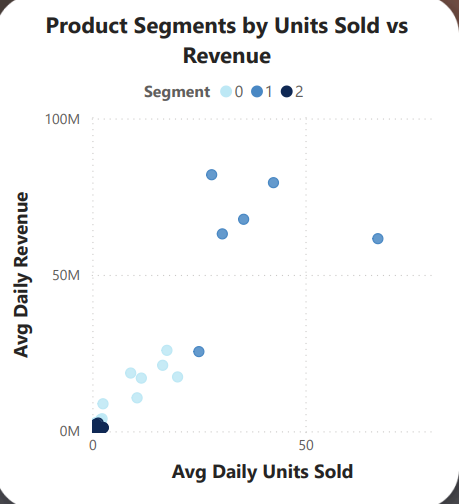
\includegraphics[width=\linewidth]{images/5.2 (1).png}
        \caption{Product segments by units sold vs revenue}
    \end{subfigure}
    \hfill
    \begin{subfigure}[t]{0.48\textwidth}
        \centering
        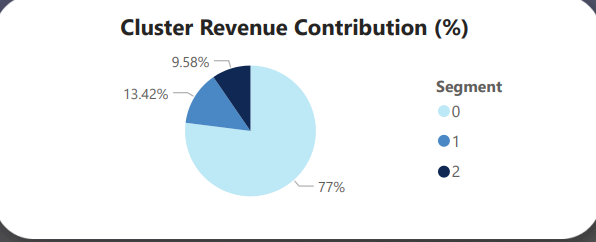
\includegraphics[width=\linewidth]{images/5.2 (2).png}
        \caption{Cluster revenue contribution}
    \end{subfigure}
    \caption{Cluster contribution to overall sales performance}
\end{figure}

\begin{itemize}[leftmargin=*, label=\textbullet]
    \item \textbf{Mark:} Points in the scatter plot and pie slices in the contribution chart.
    \item \textbf{Channel:} The scatter plot uses spatial position to compare performance by units sold and daily revenue, while the pie chart uses slice area and color to show each segment's share of total revenue.
    \item \textbf{Rationale:} These charts were chosen because Objective 5.2 asks not only how clusters differ, but also how much each cluster contributes to overall sales performance. The scatter plot explains the behavioral profile of each segment, while the pie chart directly answers the contribution question by showing revenue share across clusters.
    \item \textbf{Insight:} Segment \textbf{0} contributes the largest share of total revenue at about \textbf{77\%}, so the mainstream product group remains the main commercial base of the portfolio. The remaining segments contribute about \textbf{13.42\%} and \textbf{9.58\%}, which shows that smaller groups still matter but play more specialized roles. Combined with the scatter plot, this indicates that overall revenue is dominated by the broad central segment rather than by the extreme high-performing or low-performing groups alone.
\end{itemize}

\subsection{Overall Summary of Findings}

The objective-based visual analysis supports the group's common analytical problem in a coherent way. Category revenue is concentrated in a few strong groups, the portfolio's financial center lies in the 1M--3M VND range, and product influence is shaped by several standout items with visible mid-March spikes. Customer review volume changes more strongly than average rating, while the clustering layer shows that the catalog can be meaningfully separated into segments with different performance profiles and different revenue contributions.

Overall, the report now aligns the analysis narrative directly with the dashboard evidence used in the final submission. This makes Section 3 more consistent with the actual visuals, easier to defend in presentation, and more clearly connected to the measurable objectives introduced in Section 1.
